\title{KKRnano: Density Functional Theory application for a million atoms}
\author{
        Marcel Bornemann, IAS-1, Forschungszentrum J{\"u}lich
        \and
        Paul F.~Baumeister, JSC, Forschungszentrum J{\"u}lich
         \and
        Rudolf Zeller, IAS-3, Forschungszentrum J{\"u}lich
        }
\date{}

\maketitle

\section*{Description of the Code} 

KKRnano is a Density Functional Theory (DFT) application optimized 
for the treatment of thousands of atoms.
Standard DFT methods are usually limited to a few hundred atoms because of
their cubic scaling behaviour of the runtime caused by the need for matrix diagonalizations.
Our approach is based on matrix inversion rather than diagonalizations. 
Here, direct matrix inversions are avoided and replaced by
an iterative scheme known as transpose-free quasi-minimal residual method (tfQMR).
With this and a cut-off of atomic interactions beyond a certain distance
the computational complexity can be reduced to scale linearly 
with the number of atoms in the system.\cite{zeller_towards_2008,kkrnano:thiess_massively_2012}
\\
The application is implemented in Fortran90 and supports hybrid parallelization 
using MPI and OpenMP.
The tested version of KKRnano exclusively uses MPI collectives and two-sided MPI communication calls.
Compute-intense linear algebra operations are performed by calling BLAS/LAPACK routines wherever applicable.
File I/O is required only at application startup and after the convergence of the self-consisteny cycle.
For long runs, additional creations of checkpoints on the disk are being discussed. 
As of now, I/O operations are realized using Fortran direct-access files but an upgrade to MPI I/O is planned.
\\
The current scientific focus of KKRnano lies on large-scale magnetic structures.
For example the helical magnet MnGe in B20 structure which requires a minimum of 8 atoms per unit cell 
and can easily reach supercell sizes of a million atoms when large magnetic superstructures need to be accomodated in the simulation volume.
% Another interesting material is Cu$_x$Zr$_{1-x}$, a so-called nanoglass with outstanding mechanical material properties.
% The majority of the weak and strong scaling benchmarks are performed with input data for MnGe.
We perform a series of weak scaling tests on different supercell sizes of MnGe.
Our aim for these benchmarks is to treat several thousands of atoms self-consistently, 
i.e.~estimate the runtime that about a hundred KKR iterations in a production calculation would require.
However, for the purpose of obtaining benchmark results a single KKR iteration is sufficient.
\\
As a long-term goal we plan to overcome the threshold of a million atoms.

\begin{figure}[h!]
\begin{center}
  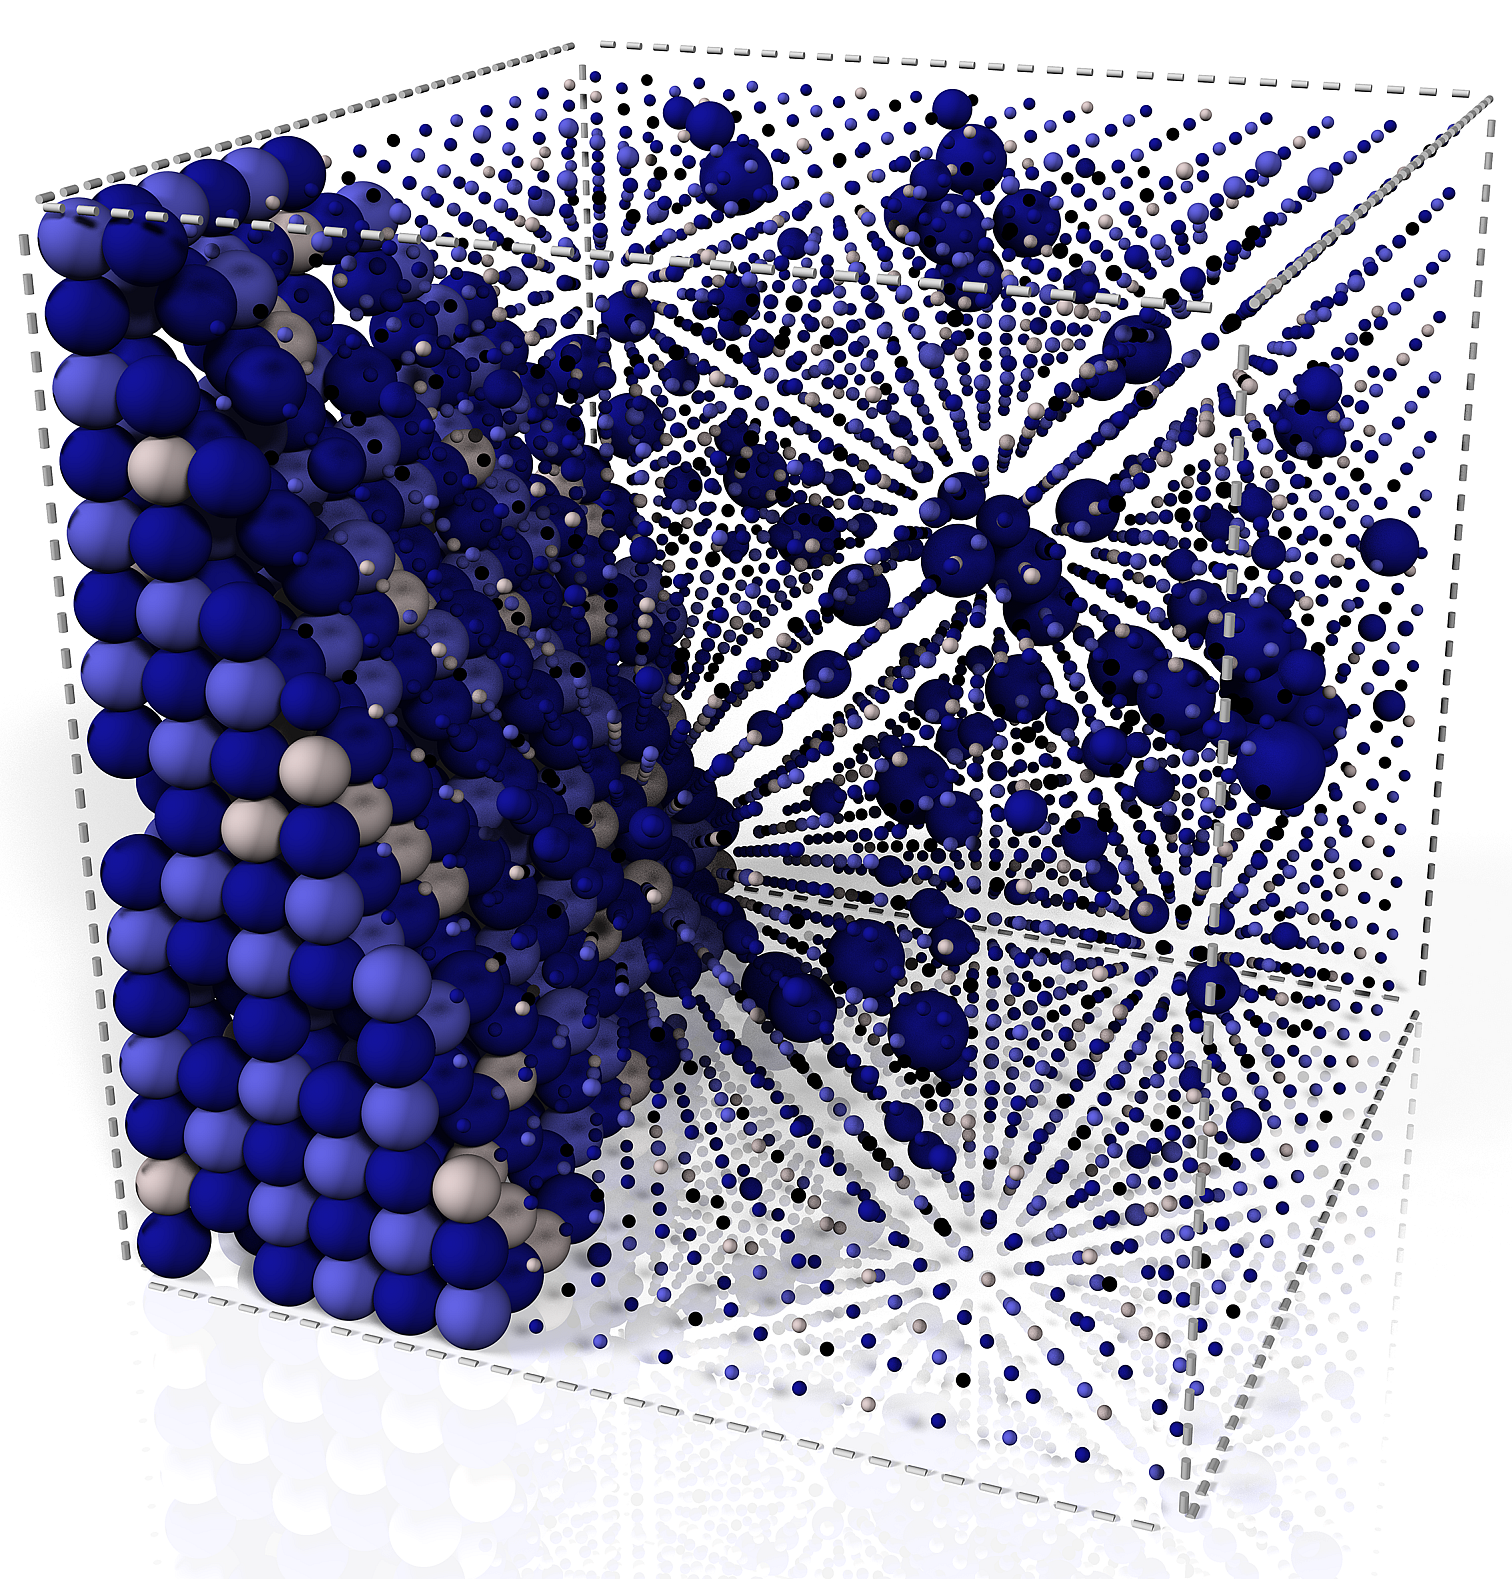
\includegraphics[width=0.6\textwidth]{NatConference.png}
  \caption{GeSbTe: A phase change material calculated with KKRnano}
\end{center}
\end{figure}

\section*{Results on MnGe} 
The weak-scaling benchmarks are performed for MnGe. KKRnano is compiled
with the IBM XL compiler (-q64,-O3,-qstrict) and linked to the ESSLSMP linear algebra package.
Here, three different hybrid parallelization schemes are used:
\begin{itemize}
 \item The first runs are conducted with a task distribution of $16$ MPI processes per node 
and $4$ OpenMP threads per process (see Tab.~\ref{kkrnano:mnge_weakscaling_moderateomp}).
This setup is supposed to work best as it complies with the vendor's suggestion.
% did we check that the 4 threads end up on the same core? MB: I did not and probably there is
% no way to check this now, is there?
 \item Then, OpenMP threading is increased while the number of MPI processes is lowered. 
The total number of threads running (MPI $\times$ OpenMP) is kept constant at $64$ matching 
the number of available hardware threads per node 
(see Tab.~\ref{kkrnano:mnge_weakscaling_balancedomp} and \ref{kkrnano:mnge_weakscaling_massiveomp}).
\end{itemize}
The atomic supercells are scaled from $8,192$ atoms (bg\_size$=$1024) to $229,376$ atoms (bg\_size$=28672$)
according to the number of racks used.
A physically correct description requires coverage of the magnetic properties of MnGe, 
i.e.~both a spin-up and a spin-down calculation need to be done. Thus, we start twice as many MPI tasks as 
are needed to treat the non-magnetic system,
e.g.~for $8192$ atoms in a $16 \times 8 \times 8$-supercell $16,384$ MPI ranks are used in \ref{kkrnano:mnge_weakscaling_moderateomp}.
%
Runtimes are measured for the initialization, a single self-consistency iteration and result output.
Each MPI process reads four \textbf{shared} binary direct-access files before commencing the self-consistency iterations. 
Two of them are index-files of the size of a few hundred kByte while the other two can grow with system size up to several GByte.
The combined size of all files that are read in is roughly $N \times 0.5\,$MBytes, where $N$ is the number of atoms.
In our benchmarks we do not write out a converged potential as we perform only a single self-consistency step.
However, a single \textbf{shared} index file is set up at the very beginning before the self-consistency loop. 
This and the read-in of the four files mentioned above accounts for most of the time spent in I/O.
In order not to hit the walltime limit for test runs of one hour,
writing of the index file is ommited in the calculations on $24$ and $28$ racks, indicated with a (t)
in Tab.~\ref{kkrnano:mnge_weakscaling_moderateomp}.
\\
Figure \ref{kkrnano:mnge_weakscaling_total} shows the total runtime of a single self-consistency iteration 
for all three parallelization concepts in a double logarithmic plot. 
Obviously, a bipartite distribution of MPI and OpenMP load promotes shorter runtimes.
We know from timing output that the increased slope for $8$ racks and higher can be mainly attributed 
to Fortran direct-access I/O which does not scale well on a GPFS file system.
%% we have all the timings, why do we have to guess here? You are right, we do not need to write 'believe'.
The observation that the increase in runtime when moving from $8$ to $28$ racks
is linked to the number of MPI tasks is a strong hint to this
as the amount of file accesses is proportional to the number of MPI processes.
The implementation of a more suitable I/O library (e.g., MPI I/O or SIONlib) is likely to solve this issue. 
\\
The tfQMR solver is expected to account for most of the computational work in KKRnano
which is why linear scaling is of particular importance in this part of the code. 
Timings for it are depicted in Fig.~\ref{kkrnano:mnge_weakscaling_tfqmr_electrostatics} (solid lines).
Necessary MPI communication before the tfQMR part takes less than a second and is therefore
not discussed here.
%%% this sentence is unattached!:
% As mentioned briefly in the introduction, linear scaling is achieved by truncating atomic interactions beyond a certain cut-off radius.
%% how large was the truncation radius (in \AA preferably) cutoff_radius = 3.03*alat = 3.03*9.06123 a_0 = 14,53 \AA 
Our benchmark results suggest to use a more MPI-oriented parallelization architecture in order to
achieve best performance.
% However, it should be noted that OpenMP is of particular importance
% if there are considerably less available hardware threads than there are atoms in the unit cell.
% In such a scenario a single MPI task handles multiple atoms and
% benefits from vectorization in BLAS Level 3 routines as matrix-vector operations become matrix-matrix operations.
% This approach also drastically improves the time-to-solution ratio.
However, it should be noted that the tfQMR solver kernel has been restructured
to benefit from OpenMP threads. Shifting from one atom per MPI process towards
e.g.~$8$ atoms per process reduces the memory requirements for the operator to
be inverted as neighboring atoms can share matrix elements.
Also the solver performance should increase using more OpenMP threads and thes ranks per node, 
however, this effect cannot be observed here. A more thourough investigation and 
architecture-specific tuning would be needed.
\\
In the KKR formalism, the electron density and the potential are connected via the Poisson equation. 
For large systems the Poisson solver contributes considerably to the overall runtime
(see dashed lines in Fig.~\ref{kkrnano:mnge_weakscaling_tfqmr_electrostatics}). 
This is expected since the algorithm used in KKRnano scales quadratically with the number of atoms 
but does not have a major impact when mid-sized systems are investigated.
However, there are ideas on how to restructure the Poisson solver towards a more favorable scaling behavior.
This is very likely planned for the near future.
\\
In order to get a more realistic impression, we extraploated the total runtime
for more than one self-consistency iteration. The extrapolated results for $10$ iterations can be found in Fig.~\ref{kkrnano:mnge_weakscaling_10SCF_iterations}.
Here, the black line is not connecting between $16$ and $24$ racks as the bottleneck of final I/O
has been omitted in the two calculations with $393,216$ and $458,752$ MPI ranks on $24$ and $28$ racks, respectively.
As mentioned above, production runs may have of the order of hundred iterations.
Multiplying the runtimes with a factor $100$ would for some test cases exceed a walltime of one day.

%%% directories:
% drwx------ 9 pbaum zam     512 Jan 24 22:25 MnGeB20_weakscaling_cubic			--> 16 MPI processes *  4 OpenMP threads
% drwx------ 9 pbaum zam     512 Jan 25 14:47 MnGeB20_weakscaling_cubic_fairomp		-->  8 MPI processes *  8 OpenMP threads
% drwx------ 9 pbaum zam     512 Jan 24 22:31 MnGeB20_weakscaling_cubic_massiveomp	-->  1 MPI processes * 64 OpenMP threads
%%% not considered
% drwx------ 9 pbaum zam     512 Jan 25 13:42 MnGeB20_weakscaling_cubic_moderateomp	-->  4 MPI processes * 16 OpenMP threads all crashed


\begin{figure}[h!]
\begin{center}
  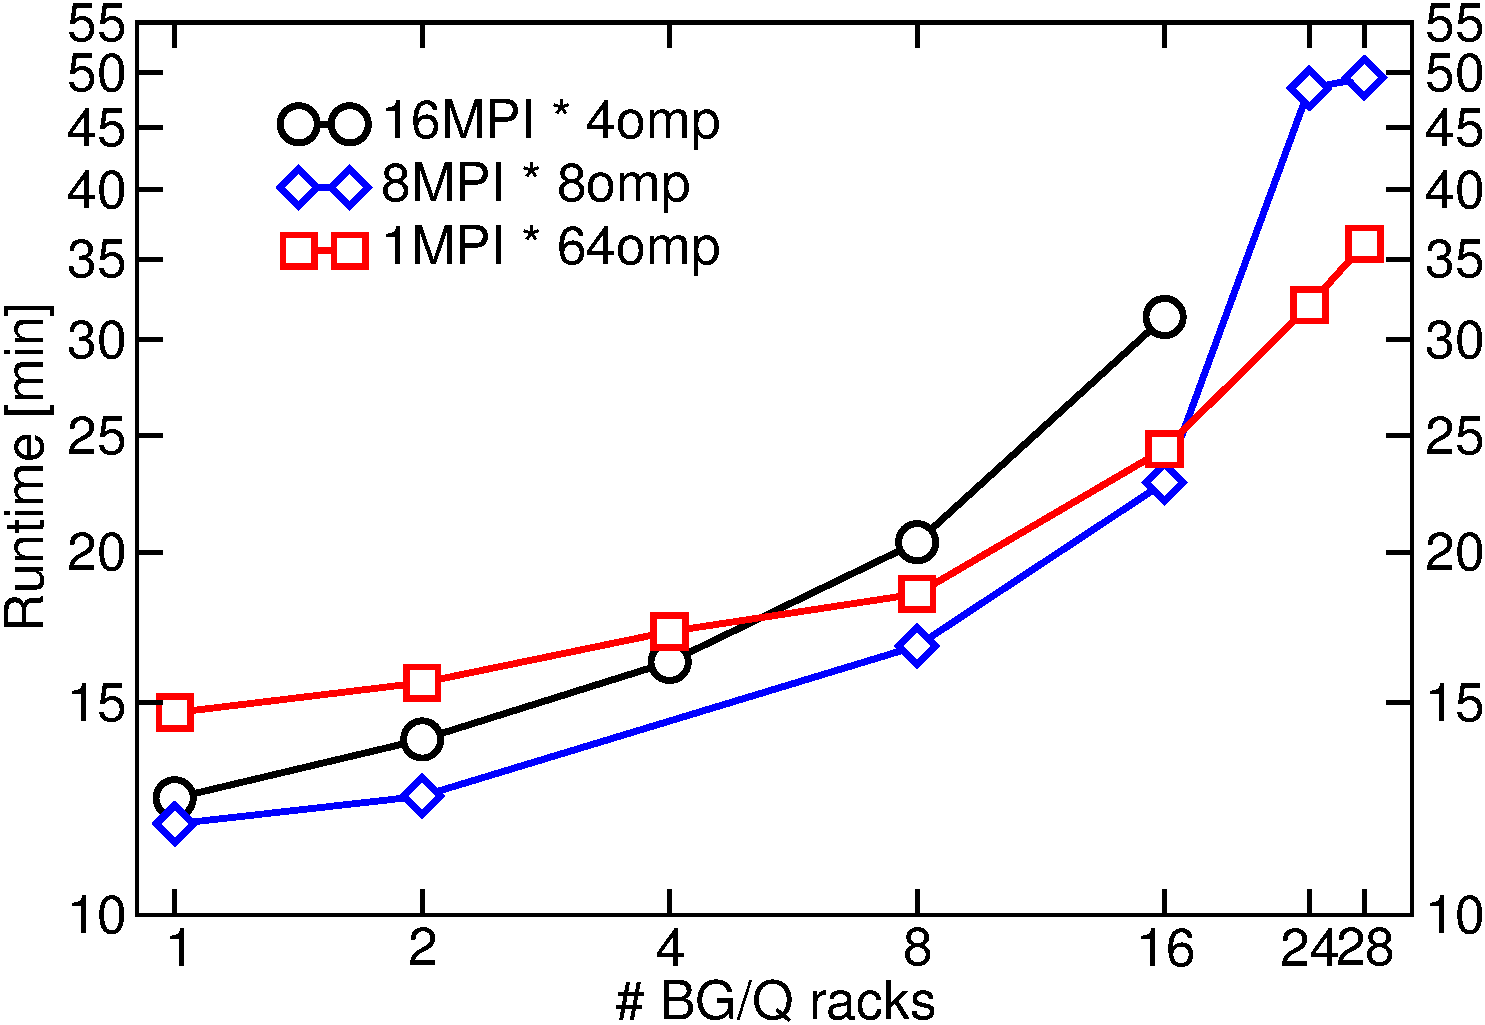
\includegraphics[width=1.0\textwidth]{results/total_runtimes.pdf}
  \caption{Weak scaling of the total runtime for a single SCF iteration on MnGe using $1$ to $16$ BG/Q racks and three different parallelization schemes.}
  \label{kkrnano:mnge_weakscaling_total}
\end{center}
\end{figure}


\begin{figure}[h!]
\begin{center}
  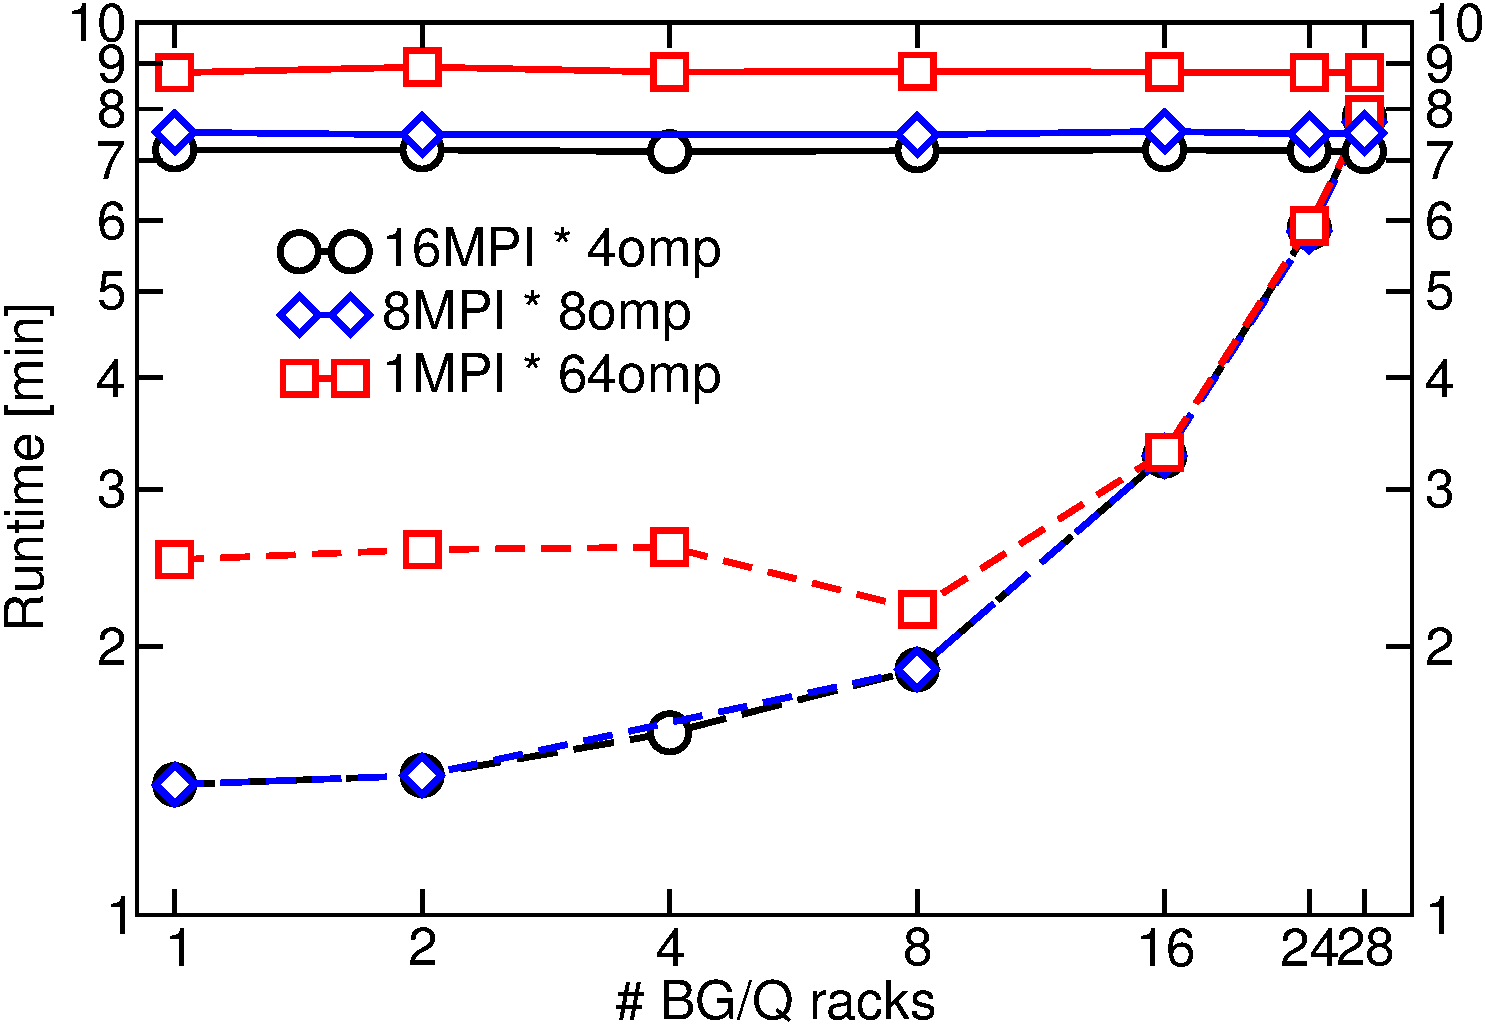
\includegraphics[width=1.0\textwidth]{results/combinedtfqmrelectrostatics.pdf}
  \caption{MnGe: Time per iteration spent in the tfQMR solver (solid lines) and in the electrostatics solver (dashed lines).}
    \label{kkrnano:mnge_weakscaling_tfqmr_electrostatics}
\end{center}
\end{figure}

\begin{figure}[h!]
\begin{center}
  \includegraphics[width=1.0\textwidth]{results/runtime_estimate_100SCF_iterations.pdf}
  \caption{Extrapolated weak scaling of the total runtime for $10$ SCF iterations on MnGe. 
  The triangles indicate the two runs with no final I/O operations.}
  \label{kkrnano:mnge_weakscaling_10SCF_iterations}
\end{center}
\end{figure}


\begin{table}[h!]
  \caption{Total runtime (Total), tfQMR solver runtime (tfQMR) and electrostatics solver runtime (ES)
  in weak scaling measurement series employing moderate OpenMP parallelization
  with $16$ MPI ranks per node and $4$ threads per process. 
  Runtimes are given in seconds. (t) indicates the tuned version where final I/O is omitted.}
\begin{center}
\begin{tabular}{|c|r|r|r|r|r|r|}
\hline
 Supercell               & bg\_size & MPI ranks &   Threads &    Total & tfQMR &  ES \\
\hline\hline
$16 \times  8 \times  8$ &  1,024   &  16,384   &    65,536 &      750 &   432 &  84 \\
$16 \times 16 \times  8$ &  2,048   &  32,768   &   131,072 &      839 &   432 &  86 \\
$16 \times 16 \times 16$ &  4,096   &  65,536   &   262,144 &      973 &   430 &  96 \\
$32 \times 16 \times 16$ &  8,192   & 131,072   &   524,288 &     1223 &   431 & 113 \\
$32 \times 32 \times 16$ & 16,384   & 262,144   & 1,048,576 &     1880 &   432 & 196 \\
$32 \times 32 \times 24$ & 24,576   & 393,216   & 1,572,864 & (t) 1077 &   431 & 353 \\
$32 \times 32 \times 28$ & 28,672   & 458,752   & 1,835,008 & (t) 1210 &   430 & 470 \\
\hline
\end{tabular}
\end{center}
\label{kkrnano:mnge_weakscaling_moderateomp}
\end{table}

\begin{table}[h!]
  \caption{Total runtime (Total), tfQMR solver runtime (tfQMR) and electrostatics solver runtime (ES)
  in weak scaling measurement series employing balanced OpenMP parallelization
  with $8$ MPI ranks per node and $8$ threads per process. Runtimes are given in seconds.}
\begin{center}
\begin{tabular}{|c|r|r|r|r|r|r|}
\hline
 Supercell               & bg\_size & MPI ranks &   Threads & Total & tfQMR &  ES \\
\hline\hline
$16 \times  8 \times  8$ &  1,024   &   8,192   &    65,536 &   714 &   452 &  84 \\
$16 \times 16 \times  8$ &  2,048   &  16,384   &   131,072 &   753 &   449 &  86 \\
$16 \times 16 \times 16$ &  4,096   &  32,768   &   262,144 &   --- &   --- & --- \\
$32 \times 16 \times 16$ &  8,192   &  65,536   &   524,288 &  1003 &   449 & 113 \\
$32 \times 32 \times 16$ & 16,384   & 131,072   & 1,048,576 &  1371 &   453 & 196 \\
$32 \times 32 \times 24$ & 24,576   & 196,608   & 1,572,864 &  2910 &   450 & 350 \\
$32 \times 32 \times 28$ & 28,672   & 229,376   & 1,835,008 &  2969 &   451 & 464 \\
\hline
\end{tabular}
\end{center}
\label{kkrnano:mnge_weakscaling_balancedomp}
\end{table}

\begin{table}[h!]
  \caption{Total runtime (Total), tfQMR solver runtime (tfQMR) and electrostatics solver runtime (ES)
  in weak scaling measurement series employing massive OpenMP parallelization with $1$ MPI rank per node
  and $64$ threads per process. Runtimes are given in seconds.}
\begin{center}
\begin{tabular}{|c|r|r|r|r|r|r|}
\hline
 Supercell               & bg\_size  & MPI ranks  &   Threads & Total & tfQMR &  ES \\
\hline\hline
$16 \times  8 \times  8$ &     1,024 &      1,024 &    65,536 &   883 &   527 & 150 \\
$16 \times 16 \times  8$ &     2,048 &      2,048 &   131,072 &   935 &   535 & 154 \\
$16 \times 16 \times 16$ &     4,096 &      4,096 &   262,144 &  1031 &   528 & 155 \\
$32 \times 16 \times 16$ &     8,192 &      8,192 &   524,288 &  1108 &   529 & 132 \\
$32 \times 32 \times 16$ &    16,384 &     16,384 & 1,048,576 &  1461 &   528 & 198 \\
$32 \times 32 \times 24$ &    24,576 &     24,576 & 1,572,864 &  1923 &   527 & 355 \\
$32 \times 32 \times 28$ &    28,672 &     28,672 & 1,835,008 &  2162 &   527 & 473 \\
\hline
\end{tabular}
\end{center}
\label{kkrnano:mnge_weakscaling_massiveomp}
\end{table}


% \section*{Results on CuZr} 

%%% to be written


\section*{Conclusion}
The participation in the 2017 JUQUEEN Extreme scaling workshop gave us the opportunity to test KKRnano on a large scale and
analyse its behaviour under such conditions.
While we already had an idea of where potential bottlenecks could be, we are now able
to quantify them and rearrange our priorities with regards to tuning and further optimization.

% -- optional
%\section*{Acknowledgments}

\bibliographystyle{plain}
\begin{thebibliography}{10}
\bibitem{zeller_towards_2008} Zeller, Rudolf.;
   \textit{Towards a linear-scaling algorithm for electronic structure calculations with the tight-binding Korringa-Kohn-Rostoker {Green} function method};
    Journal of Physics: Condensed Matter \textbf{20} (2012) 294215;
    [DOI: 10.1088/0953-8984/20/29/294215]
\bibitem{kkrnano:thiess_massively_2012} Thiess, A. and Zeller, R. and Bolten, M. and Dederichs, P. H. and Bl{\"u}gel, S.;
   \textit{Massively parallel density functional calculations for thousands of atoms: {KKRnano}};
    Physical Review B \textbf{85} (2012) 235103;
    [DOI: 10.1103/PhysRevB.85.235103]
\end{thebibliography}
